\section*{Risultati}
In questa sezione sono esposti in primo luogo i risultati delle analisi condotte sui singoli campioni e in seguito le considerazioni prodotte dal confronto tra quest'ultimi. 

L'analisi dei tempi di rilassamento per i due campioni ha previsto l'elaborazione dei dati attraverso il software UPENWin.

Per valutare con maggior consistenza i risultati il software è stato eseguito sugli stessi dati dei campioni secondo diverse configurazioni.

Le configurazioni impostate per Upen riguardo ai dati del tuorlo e dell'albume sono state, eccetto la configurazione di default, l'utilizzo del doppio e del triplo dei punti a disposizione per formulare la soluzione quasi-continua o, in alternativa, la variazione del parametro di smoothing. 
Le specifiche delle configurazioni sono citate in seguito. 

Le prime due sezioni sono suddivise in due parti: la prima relativa all'analisi del tempo di rilassamento longitudinale $T_1$, che ha coinvolto la tecnica di Inversion Recovery, e la seconda relativa al tempo di rilassamento trasversale $T_2$, che ha coinvolto la tecnica di CPMG. 



\subsection*{Albume} 

Riguardo all'albume, dall'analisi sul tempo di rilassamento longitudinale $T_1$, i cui valori sono riportati nella prima colonna della tabella \ref{tab:Albume}, sono rilevati due intervalli di tempo i cui segnali non sono trascurabili. 

Tali risultati sono confermati da un'analisi qualitativa dei grafici(\ref{subfig:T_1albume}), vista la presenza simultanea di un picco principale e un secondo picco con intensità di segnale inferiore di almeno due ordini di grandezza. 
In particolare il secondo piccolo è individuato ad un tempo di rilassamento più piccolo, indicando la presenza di un composto diverso dall'albume.

Questo secondo picco è sottolineato nelle configurazioni di oversmoothing di Upen sia per valori del coefficiente di smoothing vicini a 1 che prossimi a 10 e ciò rafforza l'ipotesi della presenza di una piccola impurità all'interno dell'albume. 

Per quanto riguarda il tempo di rilassamento trasversale $T_2$, il cui valore è stimato nella seconda colonna della tabella \ref{tab:Albume}, sia l'analisi qualitativa dei grafici(\ref{subfig:T_2albume}) che l'analisi quantitativa riportano un comportamento molto simile con $T_1$.

Anche in questo caso è possibile notare dai dati la presenza di un picco più intenso e di un secondo piccolo a tempi di rilassamento piccoli, che supporta l'ipotesi di impurità nel campione.

Sia per $T_1$ che per $T_2$ la larghezza dei picchi è stretta e ciò ad indicare come i composti siano nelle stesse condizioni. 

\begin{figure}[h]
\centering
\subfloat[][\emph{$T_1$ albume.}]
	{\label{subfig:T_1albume}
	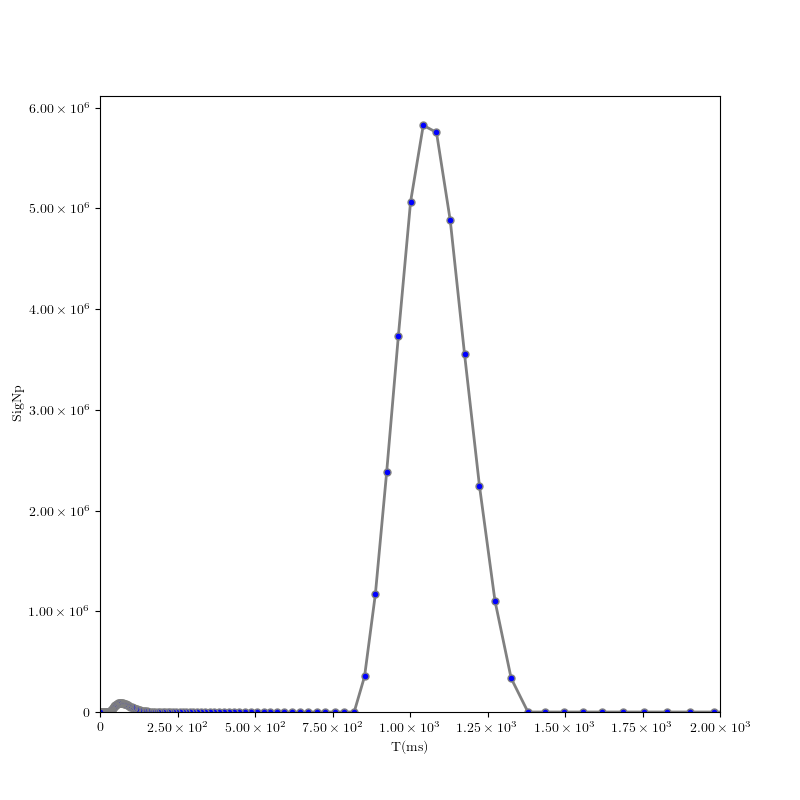
\includegraphics[scale=.25]{IRalbumeTriplo.png}
	} \quad
\subfloat[][\emph{$T_2$ albume.}]
	{\label{subfig:T_2albume}
	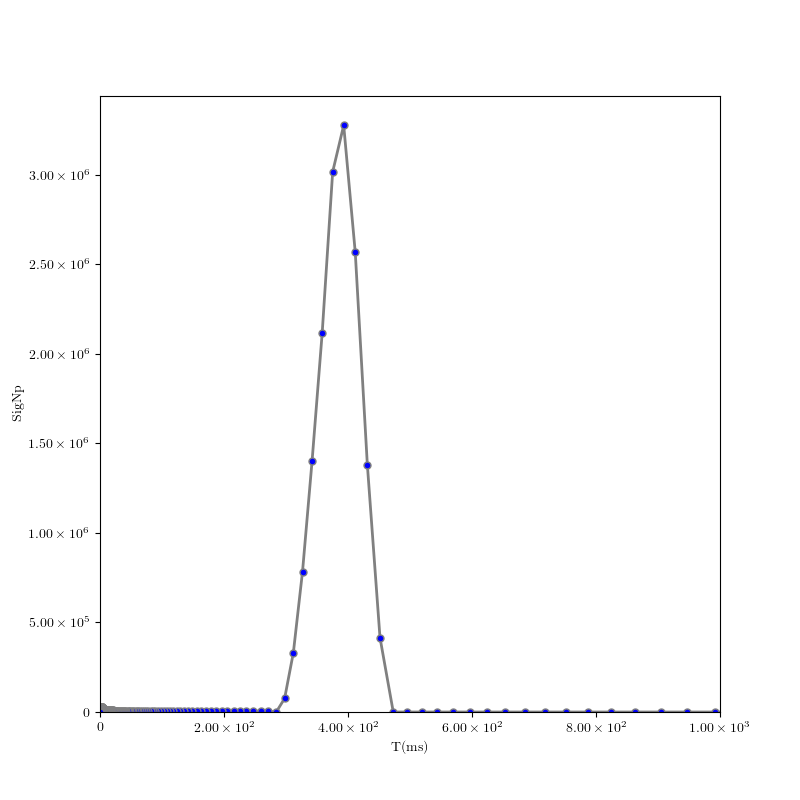
\includegraphics[width=.42\textwidth]{CPMGalbume1Triplo.png}
	} \\
\caption{}
\label{fig:T_albume}
\end{figure}

Entrambe le curve nel grafico sono state delineate a partire dai dati generati da Upen nella configurazione contenente il triplo dei dati grezzi a disposizione.
\'E stato scelto questo grafico tra tutti quelli ricavati poichè è stato considerato il più rappresentativo.

\begin{table}[h]
	\centering
	\begin{tabular}{ccc}
	\toprule
					\textbf{Albume}	\\
		$T_1\,(ms)$ 		& 		$T_2\,(ms)$ 		\\	
	\midrule
		$1000\,\pm\,300$	&		$400\,\pm\,160$		\\
		$65\,\pm\,100$		&		$4\,\pm\,12$		\\
	\bottomrule
	\end{tabular}
	\caption{Stime dei tempi di rilassamento $T_1$ e $T_2$ dell'albume.}
	\label{tab:Albume}
\end{table}

Le stime dei valori dei tempi di rilassamento sono state calcolate mediando i valori relativi al punto con maggiore intensità di segnale tra tutte le configurazioni considerate.

L'errore associato ai valori è stato invece calcolato come semidispersione della larghezza del picco nella configurazione con massima larghezza.
Conseguentemente le stime dei tempi sono accompagnate da errori molto elevati, in alcuni casi anche maggiori del valore stesso, ma ciò è ammissibile vista l'assenza di un metodo generale adeguato per la stima del migliore errore da associare a tale misura.

Studiando la relazione tra i tempi di rilassamento dell'albume, tramite una normalizzazione sui dati, è possibile evidenziare come il tempo di rilassamento $T_2$ sia molto minore rispetto a $T_1$;
ciò a riprova del fatto che il fluido è più viscoso dell'acqua.   
Il grafico seguente \ref{fig:Albume} rappresenta tale evidenza.

\begin{figure}[h]
\centering
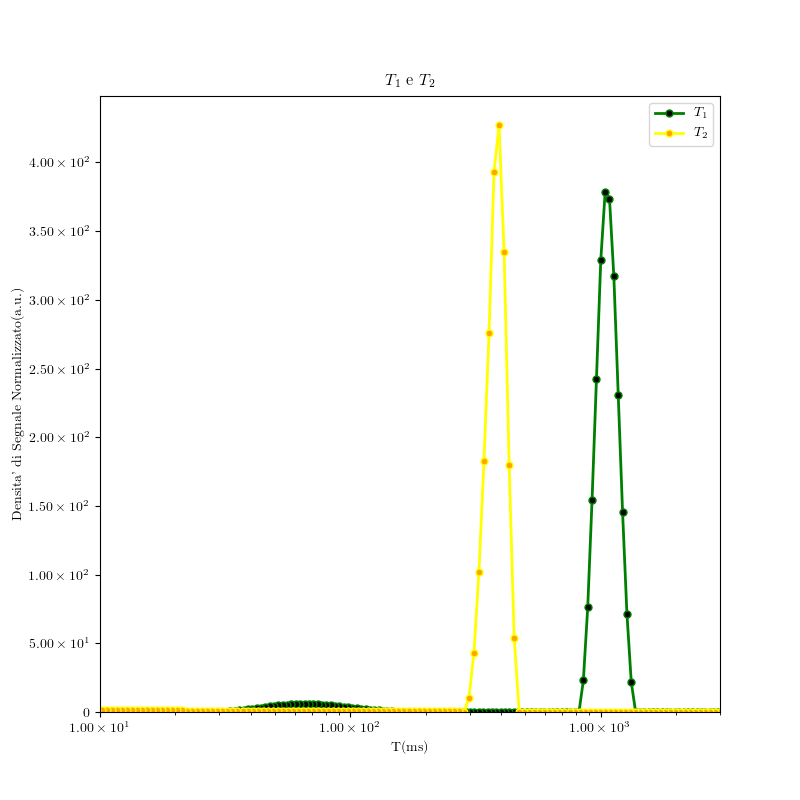
\includegraphics[scale=0.25]{T_albume_merge.png}
\caption{Relazione tra la densità di segnale normalizzato e i tempi di rilassamento per il campione di albume.}
\label{fig:Albume}
\end{figure}




\subsection*{Tuorlo}

Le analisi condotte sul tuorlo hanno riportato un andamento differente da quello dell'albume.
I grafici descritti per il tempo di rilassamento $T_1$ contengono un picco pronunciato che per alcune configurazioni ha una coda allungata e per altre si separa da un altro picco meno intenso.
Infatti, per le configurazioni di Upen di default e di oversmoothing risulta chiaro quest'ultimo effetto; mentre considerando il doppio e il triplo dei dati grezzi, oltre al caso di undersmoothing, il picco è dotato di una coda allungata verso tempi maggiori.

I dati relativi a $T_1$ si possono trovare nella prima colonna della tabella \ref{tab:Tuorlo} mentre è possibile visualizzare una curva rappresentativa nel sottografico \ref{subfig:T_1tuorlo}. 

Lo studio sul tempo di rilassamento $T_2$ sul campione di tuorlo condivide invece alcuni dei risultati che sono stati ottenuti per l'albume. 
Come per quest'ultimo infatti, è presente un picco principale e un abbozzamento a tempi inferiori con intensità nettamente inferiore ma, come per il $T_1$, per valori di tempi maggiori del picco principale la curva descrive un andamento più incerto.
Infatti, come nel caso precedente per alcune configurazioni si manifesta un altro picco e per altre un allungamento della coda.

Un andamento di questo tipo evidenzia che, visto l'allargamento del picco, sono presenti altri composti.
In tale caso l'effetto è più evidente e i dati consentono di ipotizzare con maggior affidabilità l'impurità del tuorlo.

I valori relativi a $T_2$ per i due picchi sono segnati nella seconda colonna della tabella \ref{tab:Tuorlo}; mentre il sottografico \ref{subfig:T_2tuorlo} delinea l'andamento più consistente.

\begin{figure}[h]
\centering
\subfloat[][\emph{$T_1$ tuorlo.}]
	{\label{subfig:T_1tuorlo}
	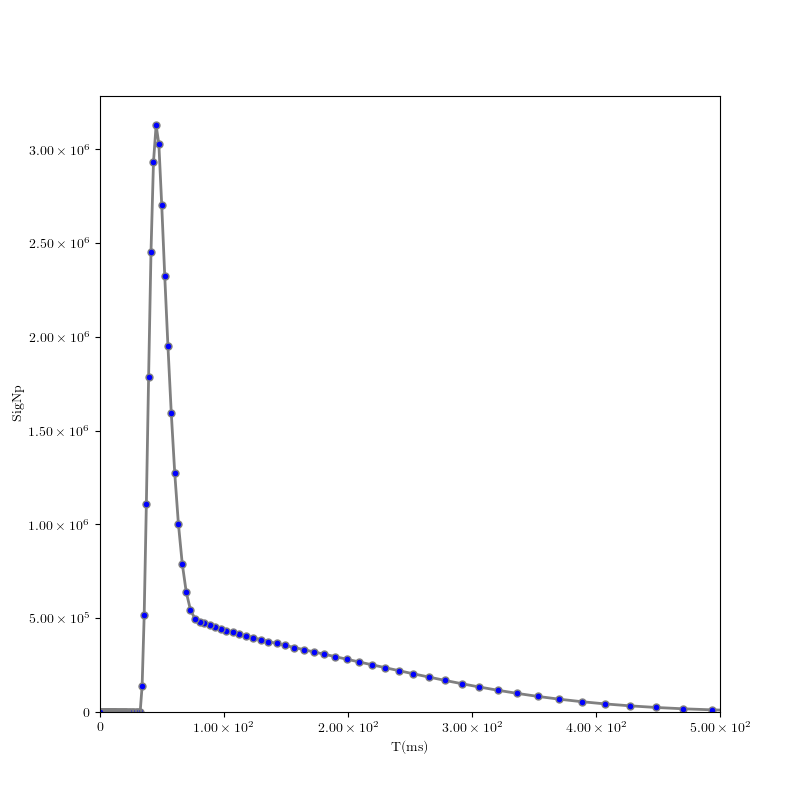
\includegraphics[scale=.25]{IRtuorloTriplo.png}
	} \quad
\subfloat[][\emph{$T_2$ tuorlo.}]
	{\label{subfig:T_2tuorlo}
	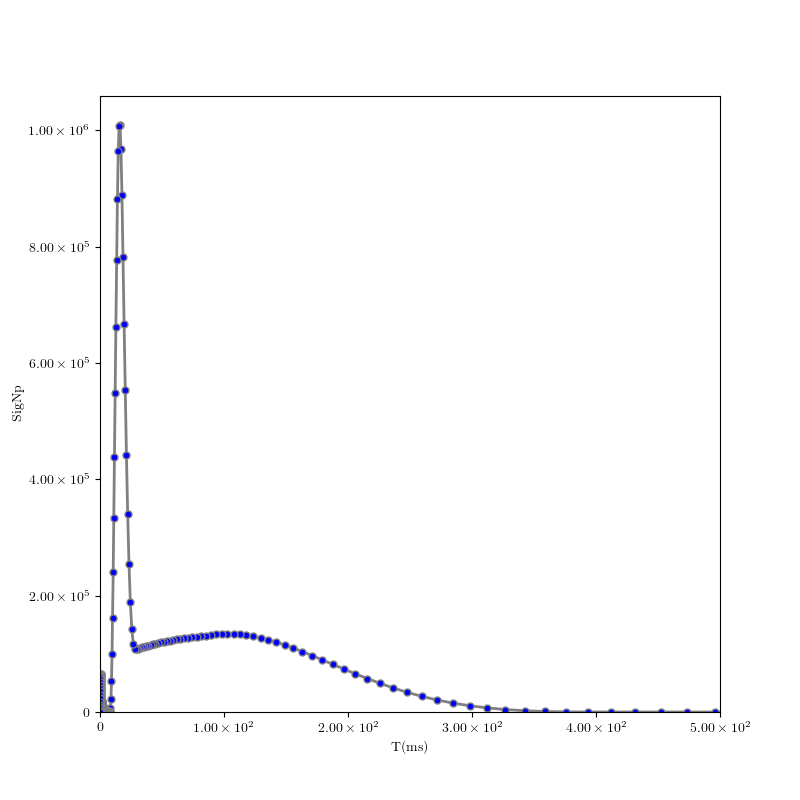
\includegraphics[width=.42\textwidth]{CPMGtuorlo1Triplo.png}
	} \\
\caption{}
\label{fig:T_tuorlo}
\end{figure}

Come per il campione d'albume anche per il tuorlo i grafici considerati sono stati derivati dalla configurazione di Upen che elabora il triplo dei dati a disposizione.

\begin{table}[h]
	\centering
	\begin{tabular}{ccc}
	\toprule
					\textbf{Tuorlo}	\\
		$T_1\,(ms)$ 		& 		$T_2\,(ms)$ 		\\	
	\midrule
		$50\,\pm\,160$	&		$16\,\pm\,13$		\\
		$100\,\pm\,400$		&		$80\,\pm\,190$		\\
	\bottomrule
	\end{tabular}
	\caption{Stime dei tempi di rilassamento $T_1$ e $T_2$ del tuorlo.}	
	\label{tab:Tuorlo}
\end{table}

Come già citato precendemente le stime sono state calcolate come media tra le varie configurazione dei valori con maggior intensità e gli errori come semidispersione della larghezza del picco nel configurazione ove tale larghezza è massima.

La relazione tra i tempi di rilassamento nel tuorlo mostrano anche i questo caso che il tempo $T_2$ è molto minore del tempo $T_1$. 
Tale risultato è meglio espresso dal grafico seguente \ref{fig:Tuorlo}.

\begin{figure}[h]
\centering
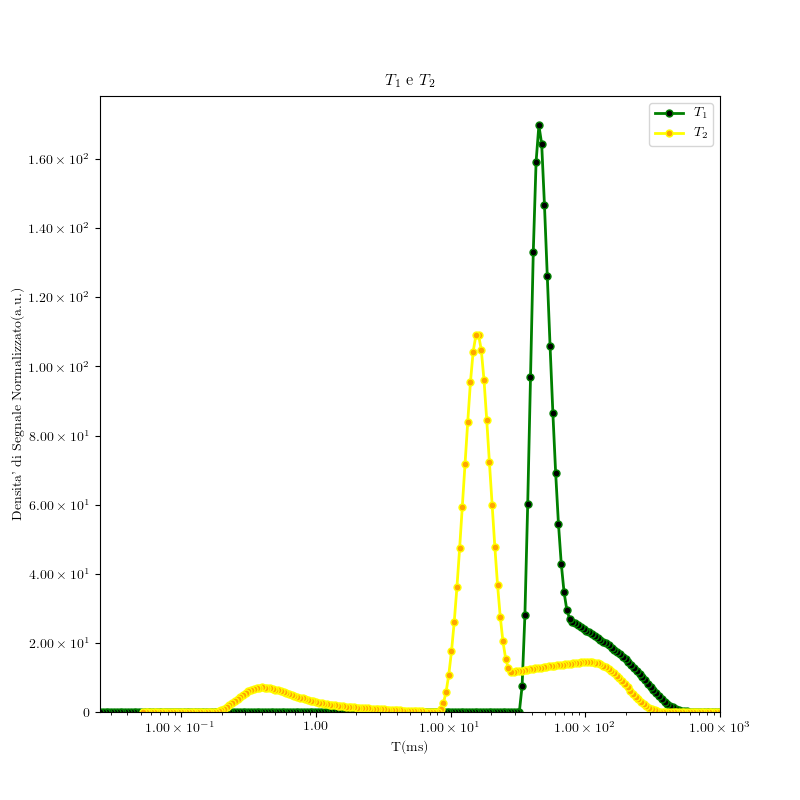
\includegraphics[scale=0.3]{T_tuorlo_merge.png}
\caption{Relazione tra la densità di segnale normalizzato e i tempi di rilassamento per il campione di tuorlo.}
\label{fig:Tuorlo}
\end{figure}


\section*{Confronto tra campioni}

La relazione tra i due campioni rivela come è possibile discriminare i due composti principali dell'uovo e come tale discriminazione può essere evidente.

Considerando i tempi di rilassamento longitudinali dal grafico \ref{subfig:T_1} è possibile osservare che il tempo associato all'albume è molto maggiore rispetto a quello misurato per il tuorlo. 
Lo stesso risultato è ottenuto dal confronto tra i tempi di rilassamento trasversali, figura \ref{subfig:T_2}.

\begin{figure}[h]
\centering
\subfloat[][\emph{Confronto tra i tempi di rilassamento longitudinali.}]
	{\label{subfig:T_1}
	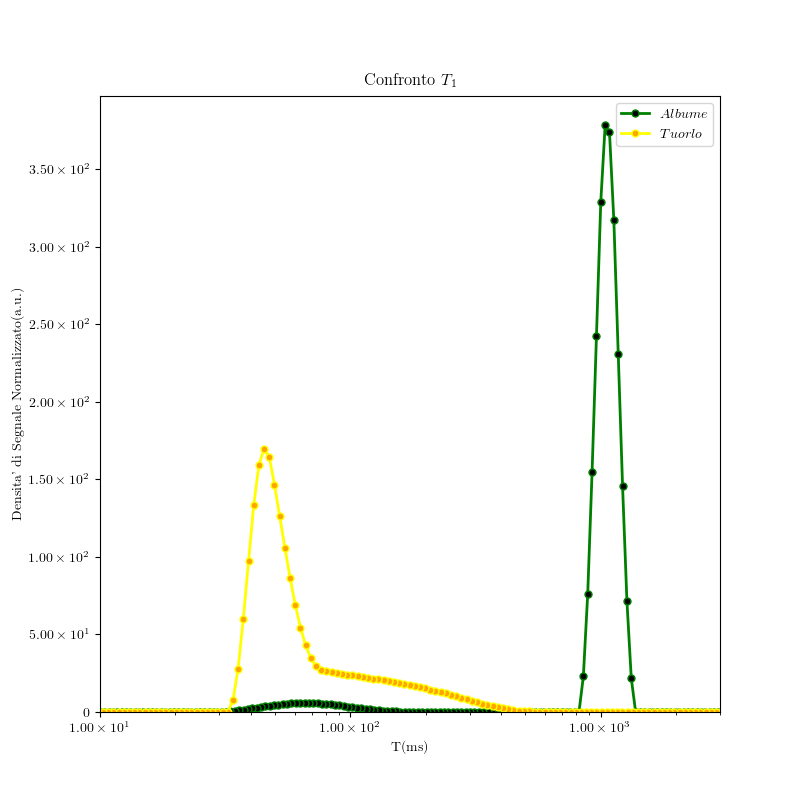
\includegraphics[scale=.25]{T_1_merge.png}
	} \quad
\subfloat[][\emph{Confronto tra i tempi di rilassamento trasversali.}]
	{\label{subfig:T_2}
	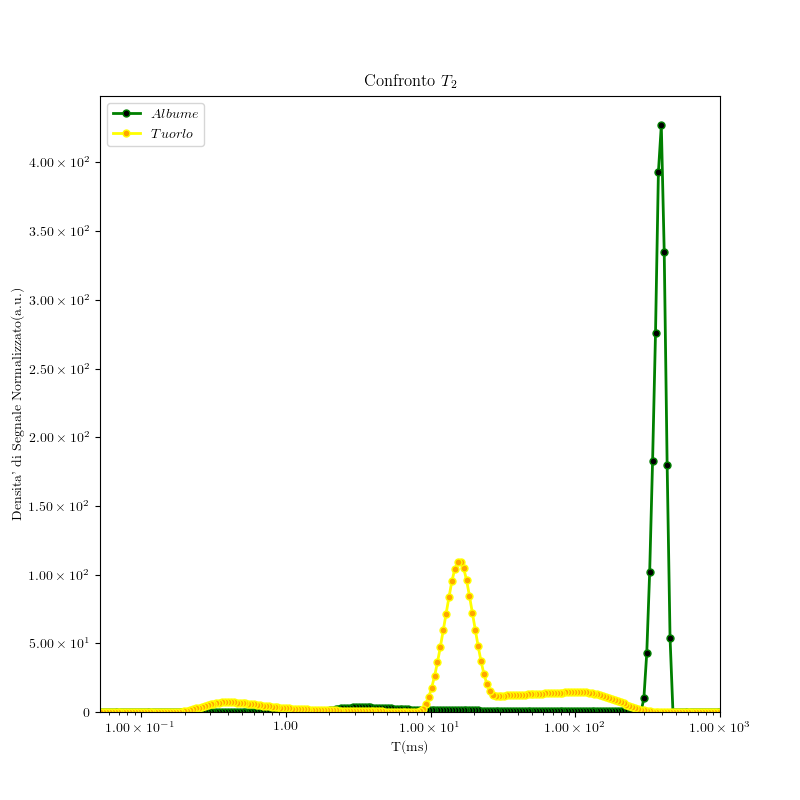
\includegraphics[width=.42\textwidth]{T_2_merge.png}
	} \\
\caption{}
\label{fig:Confronto}
\end{figure}

